\documentclass[fontsize=11pt,paper=a4]{scrartcl}

\usepackage[english]{babel}
\usepackage{microtype}
\usepackage{blindtext}
\usepackage{listings}
\usepackage{hyperref}
\usepackage{csquotes}
\usepackage{graphicx}

\lstset{
  language=C,
  basicstyle=\small,
  breaklines=true}
\frenchspacing 

%%% Maketitle metadata
\newcommand{\horrule}[1]{\rule{\linewidth}{#1}} 	

\title{
		%\vspace{-1in} 	
		\usefont{OT1}{bch}{b}{n}
		\normalfont \normalsize \textsc
		{Coursera Course: Cloud Computing} \\ [25pt]
		\horrule{0.5pt} \\[0.4cm]
		\huge Capstone Project Task 1 Report \\
		\horrule{2pt} \\[0.5cm]
}
\author{
		\normalfont 								\normalsize
        Hang Shi\\[-3pt]		\normalsize
        \today
}
\date{}


\begin{document}



\maketitle


\section{Overview}
This report covers the design and implementation details for Cloud Computing Captone Project Task 1. The goals of this task are to perform the following:
\begin{itemize}
\item Extract and clean the transportation dataset, and then store the result in HDFS.
\item Answer 2 questions from Group 1, 3 questions from Group 2, and both questions from Group 3 using Hadoop. Store the results for questions from Group 2 and Question 3.2 in Cassandra.   
\end{itemize}
 
\section{Data Cleanup}
\par The first task is to clean and store the dataset. We  first retrieve and extract the dataset from the EBS volume snapshot by following steps in \url{http://docs.aws.amazon.com/AWSEC2/latest/UserGuide/ebs-restoring-volume.html}. One key thing to note is that we need to create EC2 instance in the same region and availabbility zone as the data EBS snapshot (snap-e1608d88 in us-east-1d).   
\par Afterwards, we explore the data set and decide on how we wish to clean it. Then we ignore unrelated rows and extract only the columns from the csv files. The raw data is in \path{/data/aviation/airline_ontime} directory. 
\par Approaches: Two ways have been used to do the cleanup: 
\begin{itemize} 
\item A python script is developed on top of \href{https://docs.python.org/2/library/csv.html}{python CSV package} to achieve this. 
\item Pig script, see \url{https://pig.apache.org/} for details. 
\end{itemize}

\par Such data cleanup is a one-time job and below are the fields we extracted: 
\begin{itemize}
\item       AirlineID:chararray, --a8
\item       Carrier:chararray,   --a9
\item       FlightNum:int,       --a11
\item       Origin:chararray,    --a12       
\item       Dest:chararray,      --a18
\item       DepDelay:float,      --a26
\item       DepDel15:float,      --a28
\item       ArrDelay:float,      --a37 
\item       ArrDel15:float       --a39
\end{itemize}

\par The cleaned data are stored on HDFS via below hdfs dfs command  as tab delimetered fields with each line indicating one flight. 
\begin{lstlisting}{centered}
	hdfs dfs -copyFromLocal <local files> <hdfs dir>  
\end{lstlisting}
 
\section{System Overview}
\subsection{Hadoop MapReduce}
The system is essentially a 4 node Apache Hadoop cluster with one namenode and three datanodes running on AWS EC2. 
Hadoop Yarn runs and serves as the resource manager and application manager. Below link provides some useful information on the setup: 

\href{https://blog.insightdatascience.com/spinning-up-a-free-hadoop-cluster-step-by-step-c406d56bae42}{Spinning Up a Free Hadoop Cluster: Step by Step}


\subsection{Cassandra} 
Cassandra cluster is deployed on the three Hadoop datanodes to provide data replication and scalability. 
The cluster run on the same rack and utilizes GossipingPropertyFileSnitch scheme. One of the nodes is assigned as the seed provider.
 
\section{Group 1 Problems} 

\begin{itemize} 
\item Problem 1.1: Rank the top 10 most popular airports by numbers of flights to/from the airport.
Solution: We extracted the origin and destination city of the flight for each line of the cleaned files. It is done two steps: counting via map and reduce phases in Hadoop and sort to get top 10 airports. In the map phase, we generate pairs (origin, 1) and (dest, 1). In the reduce phase, if we see a new airport, we output the airport and count; if we see same airport, we add the count to existing counter. Once the counters are outputted, below commands can be used to get top airports (use 20 to allow duplicated top cases). 
\begin{lstlisting}[language = C++]
hadoop fs -cat /output/of/wordcount/part* | sort -n -k2 -r | head -n20
\end{lstlisting}
Alternatively, the top N problem can be solved via \href{https://github.com/adamjshook/mapreducepatterns/blob/master/MRDP/src/main/java/mrdp/ch3/TopTenDriver.java}{this MapReduce design pattern}. 

\item Problem 1.2: Rank the top 10 airlines by on-time arrival performance
In the map phase, we generate (airline, 1, delay). In the reduce phase, we use two maps: (airline, count), and (airline, total delay) and accumulate counter and delay into these two maps. Then we calculate arrival performance and sort them. Alternatively and if there are multiple reducers, we will use commands similar as in above problem to do sorting. 

\item Problem 1.3: Rank the days of the week by on-time arrival performance
This is a similar problem as Problem 1.2. We use (weekday, delay) as input data. In the map phase, we generate (weekday, 1, delay). In the reduce phase, we use two maps: (weekday, count), and (weekday, total delay) and accumulate counter and delay into these two maps. Then we calculate arrival performance and sort them.   

\end{itemize}
 
\section{Group 2 Problems}
 
\begin{itemize} 
\item For each airport X, rank the top-10 carriers in decreasing order of on-time departure performance from X.

We use Pig Latin script to generate the results into HDFS files and then store them into Cassandra database for queries. Below is the script: 

\small\begin{verbatim}
in  = LOAD '$PIG_IN_DIR' AS 
          ( AirlineID:chararray, --a8
            Carrier:chararray,   --a9
            FlightNum:int,       --a11
            Origin:chararray,    --a12       
            Dest:chararray,      --a18
            DepDelay:float,      --a26
            DepDel15:float,      --a28
            ArrDelay:float,      --a37 
            ArrDel15:float       --a39
          );
	
group_by_origin_airline = GROUP in BY (Origin, Carrier, AirlineID);

average_ontime = FOREACH group_by_origin_airline 
                 GENERATE FLATTEN(group) AS (Origin, Carrier, AirlineID), 
                          AVG(in.DepDelay) AS performance_index;

group_by_origin = GROUP average_ontime BY Origin; 
 
top_ten_airlines = FOREACH group_by_origin {
   sorted_airlines = ORDER average_ontime BY performance_index ASC;
   top_airlines = LIMIT sorted_airlines 10;
   GENERATE FLATTEN(top_airlines);
}

X = FOREACH top_ten_airlines GENERATE TOTUPLE( \
TOTUPLE( 'origin',$0), TOTUPLE( 'carrier',$1),\
TOTUPLE('airline', $2 )), TOTUPLE($3);

STORE X into '$PIG_OUT_DIR'; 
\end{verbatim}
\normalsize

\item For each airport X, rank the top-10 airports in decreasing order of on-time departure performance from X.

Below is the PIG script (table loading part is ignored). 
\small\begin{verbatim}
group_by_origin_dest = GROUP in BY (Origin, Dest);

average_ontime = FOREACH group_by_origin_dest 
                 GENERATE FLATTEN(group) AS (Origin, Dest), 
                          AVG(in.DepDelay) AS performance_index;

group_by_origin = GROUP average_ontime BY Origin; 
top_ten_airports = FOREACH group_by_origin {
   sorted_airports = ORDER average_ontime BY performance_index ASC;
   top_airports = LIMIT sorted_airports 10;
   GENERATE FLATTEN(top_airports);
}

X = FOREACH top_ten_airports GENERATE TOTUPLE( \
TOTUPLE( 'origin',$0), TOTUPLE('dest', $1 )), \
TOTUPLE($2);

STORE X into '$PIG_OUT_DIR'; 
\end{verbatim}
\normalsize

\item For each source-destination pair X-Y, rank the top-10 carriers in decreasing order of on-time arrival performance at Y from X.

Below is the PIG script (table loading part is ignored). 
\small\begin{verbatim}
group_by_origin_dest_airline = GROUP in BY (Origin, Dest, AirlineID);

average_ontime = FOREACH group_by_origin_dest_airline
               GENERATE FLATTEN(group) AS (Origin, Dest, AirlineID),
               AVG(in.ArrDelay) AS performance_index;

group_by_origin_dest = GROUP average_ontime BY (Origin, Dest);

top_ten_airlines = FOREACH group_by_origin_dest {
   sorted_airlines = ORDER average_ontime BY performance_index ASC;
   top_airlines = LIMIT sorted_airlines 10;
   GENERATE FLATTEN(top_airlines);
}

X = FOREACH top_ten_airlines GENERATE TOTUPLE( \
TOTUPLE('origin',$0), TOTUPLE('dest', $1),TOTUPLE(\
'airline', $2 )), TOTUPLE($3);

STORE X into '$PIG_OUT_DIR';
\end{verbatim}
\normalsize

%\item For each source-destination pair X-Y, determine the mean arrival delay (in minutes) for a flight from X to Y.

\end{itemize}

\section{Group 3 Problems}
\begin{itemize}
\item 1. Does the popularity distribution of airports follow a Zipf distribution? If not, what distribution does it follow?

Zipf’s law stats that given some corpus or natural language utterances, the frequency of any word is inversely proportional to its rank in the frequency table. In our case it means that the airport with a higher rank should have a double number of flights compare with the next airport in rank. Even if from the Flights by Airport figure we can hope for a Zipf distribution, after
doing a log-log plot we can see that Airports rank by number of flights is not following this distribution (log log for Zipf should be a straight line and is not). gnuplot tool is used to do plotting and it can be proven that this distribution is not Zipf but more a Lognormal one since the bottom half look very different than the top half. 

\begin{figure}
\centering
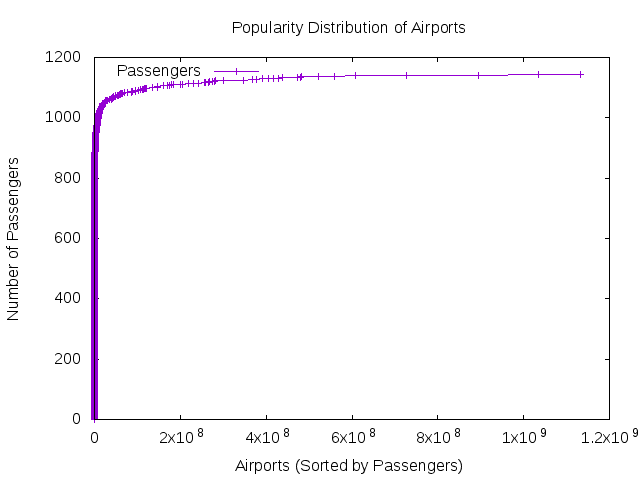
\includegraphics[totalheight=8cm]{airport_rank.png}
\caption{For poblem 3.1 Popularity Distribution of Airports.}
\label{fig:verticalcell}
\end{figure}

\item 2. Tom wants to travel from airport X to airport Z. However, Tom also wants to stop at airport Y for some sightseeing on the way. More concretely, Tom has the following requirements (see Task 1 Queries for specific queries):
\begin{itemize}
\item A. The second leg of the journey (flight Y-Z) must depart two days after the first leg (flight X-Y). For example, if X-Y departs January 5, 2008, Y-Z must depart January 7, 2008.
\item B. Tom wants his flights scheduled to depart airport X before 12:00 PM local time and to depart airport Y after 12:00 PM local time.
\item C. Tom wants to arrive at each destination with as little delay as possible.
It is solved by creating two MapReduce Jobs. One which filter the
flights by arrival performance and the second one which computes the options Tom has and pick up the best one based on arrival performance. For the first map reduce the key is based on Origin, Destination and FlightDate. In the second MapReduce we will receive a list of best arrival flights grouped by Origin-Destination-Date and from here using the 12h departure condition we can generate for each day all the options Tom has.
\end{itemize}
\end{itemize}

\section{Optimization Techniques}
\begin{itemize}
\item Removal of unused data columns: only needed columns have been imported from the original dataset, thus lowering the needs for data transfer and storage capacity.
\item Data ordering and partitioning: the import script orders and partitions by date the data from the original dataset. This way the import process into HDFS is faster.
\item Data preload into HDFS: data  is loaded to HDFS before starting to process it. This way, we can achieve persistent storage in HDFS and fast access from HDFS.
\item One optimization is to use the combiner in the map phase in order to minimize the network traffic. This is used in problems in group 1. For example, in question 1, use same reducer class as combiner class. 

\end{itemize} 
 
\section{Video Link}
To be added later. 

\end{document}
